\documentclass[10pt,a4paper]{article}
\usepackage[margin=22mm]{geometry}
\usepackage[T1]{fontenc}
\usepackage{lmodern,amsmath,amssymb,graphicx,booktabs,microtype}
\usepackage[font=small,labelfont=bf]{caption}
\usepackage[hidelinks]{hyperref}
\usepackage{fancyhdr}
\pagestyle{fancy}\fancyhf{}
\fancyhead[L]{\small Computational Mechanics Projects}
\fancyhead[R]{\small FoldTrace}
\fancyfoot[C]{\thepage}
\setlength{\headheight}{14pt}
\setlength{\parindent}{0pt}\setlength{\parskip}{5pt}
\setlength{\emergencystretch}{1em}
\newcommand{\R}{\mathbb{R}}
\title{\vspace{-1.3cm}\LARGE FoldTrace: Pseudo-Arclength Continuation Through Two Truss Limit Points}
\author{\small Computational Mechanics Projects\\\small Reproducible technical research note}
\date{\small 29 September 2026}
\begin{document}\maketitle\thispagestyle{fancy}

\begin{abstract}
Load-controlled Newton iteration becomes singular at a structural limit point. FoldTrace follows a symmetric two-bar truss through two such folds using a scaled tangent predictor and hyperplane corrector. A C++17 implementation evaluates force, consistent tangent, energy, and the augmented Newton system; Python exposes immutable path data and analytical validation. For the default height-to-span ratio 0.2, 23 accepted states cross both folds with maximum scaled equilibrium residual $7.29\times10^{-13}$. Fold locations match closed-form values within $3.34\times10^{-15}$, and step refinement gives approximately second-order path interpolation. The result is a static equilibrium curve, including unstable states, rather than a simulation of dynamic snap-through.
\end{abstract}
\section{Introduction}
At a fold, displacement ceases to be a single-valued function of load. Parameterizing by prescribed load is then unsuitable even though the equilibrium curve itself remains smooth. Path-following methods add a continuation condition to regularize this local description~\cite{riks}. FoldTrace provides a small problem for which geometry, equilibrium, tangent, energy, and fold coordinates can all be derived independently, enabling precise assessment of the numerical continuation algorithm.
\section{Geometry, equilibrium, and stability}
Supports lie at $(\pm a,0)$; an apex constrained horizontally moves to $(0,h-w)$ under downward dead load $P$. Each bar has initial length $L_0=\sqrt{a^2+h^2}$ and axial rigidity $EA$. The specified engineering-strain law is $N=EA(L-L_0)/L_0$. Define
\begin{equation}
r=h/a,\quad q=w/h,\quad \ell=\sqrt{1+r^2(1-q)^2},\quad
\ell_0=\sqrt{1+r^2},\quad\lambda=\frac{P}{2EAh/L_0}.
\end{equation}
Vertical force equilibrium and its exact tangent reduce to
\begin{equation}
R(q,\lambda)=f(q)-\lambda=0,\quad f(q)=(1-q)(\ell_0/\ell-1),
\qquad f'(q)=1-\frac{\ell_0}{\ell^3}.
\end{equation}
The dimensionless elastic energy $\bar U=U/(EAa)$ and prescribed-load potential are
\begin{equation}
\bar U=\frac{(\ell-\ell_0)^2}{\ell_0},\qquad
\bar\Pi=\bar U-\frac{2r^2}{\ell_0}\lambda q,\qquad
\bar U'=\frac{2r^2}{\ell_0}f(q).
\end{equation}
Positive $f'$ denotes a local potential minimum within the constrained symmetric degree of freedom; it does not test excluded lateral modes. Setting $f'=0$ yields
\begin{equation}
q_\pm=1\pm\sqrt{\frac{(1+r^2)^{1/3}-1}{r^2}}.
\end{equation}
These formulas supply both equilibrium and fold references without relying on a second continuation solver.
\newpage
\section{Scaled predictor--corrector method}
Use $z=(q,\lambda/s)$ with default load scale $s=r^2$. At an accepted point, normalize $(1,f'/s)$ and orient the tangent $t$ consistently with the previous step. Predict $z_p=z_n+\Delta s\,t$, then solve
\begin{equation}
F(z)=\begin{bmatrix}(f(q)-\lambda)/s\\t^T(z-z_p)\end{bmatrix}=0,
\qquad
J=\begin{bmatrix}f'/s&-1\\t_q&t_\lambda\end{bmatrix}.
\end{equation}
At a fold the tangent is horizontal, so the augmented Jacobian remains nonsingular even though $f'=0$. The constraint is a tangent hyperplane, not a spherical arc-length equation. Thus the method follows the broader continuation idea without claiming identity with every detail of the original Riks algorithm.

An attempted step is accepted only when the norm of the scaled residual pair is below tolerance, the corrector displacement is at most half the predictor length, and $q$ increases. Rejected attempts halve the step from the last accepted state. After acceptance, steps grow by 1.25 when at most three Newton updates are needed and shrink by 0.7 after seven or more, subject to bounds. This heuristic controls local continuation behavior, not a global error estimate.

The C++ kernel rationalizes length differences near $q=0$ and $q=2$ to reduce cancellation and solves the two-by-two correction system. Python validates settings and returns immutable point/path records. Failure exceptions retain the last valid partial path and report budget or minimum-step termination explicitly. The final point is an equilibrium at $q\ge q_{\rm stop}$, not an interpolated or clipped endpoint.
\section{Verification experiment}
The default study uses $r=0.2$, $s=0.04$, target $q=2.2$, initial step 0.08, maximum step 0.12, and residual tolerance $10^{-11}$. An independently evaluated force expression checks the native equilibrium result. Tangent differentiation and the force--energy identity check mechanical consistency.
\begin{center}\begin{tabular}{lr}\toprule
Recorded diagnostic & Value\\\midrule
Accepted states, including initial state & 23\\
Rejected attempts & 0\\
Maximum scaled equilibrium residual & $7.2835\times10^{-13}$\\
Maximum independent force error & $2.9160\times10^{-14}$\\
Fold coordinates $q_-,q_+$ & 0.4264278, 1.5735722\\
Maximum fold-coordinate error & $3.3307\times10^{-15}$\\
Final path-interpolation order & 2.00146\\\bottomrule
\end{tabular}\end{center}
The fold loads are $\pm0.00754787$. Halving the path step gives interpolation orders 2.02509, 2.00272, and 2.00146. These describe linear reconstruction between equilibrated points, not Newton's convergence rate and not temporal accuracy. Zero rejections in this run do not establish that all permitted parameter choices will succeed.
Figure~\ref{fig:results} visualizes selected recorded diagnostics.
\newpage
\begin{figure}[!ht]\centering
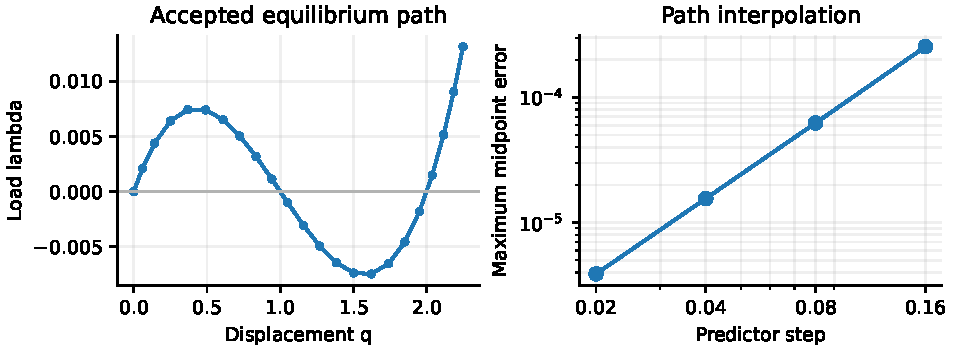
\includegraphics[width=\textwidth]{figure.pdf}
\caption{Recorded equilibrium path and path-reconstruction refinement. Negative-tangent equilibria are static mathematical states, not the time history of a snap event.}\label{fig:results}\end{figure}
\section{Discussion and limitations}
The continuation condition removes the local load-control singularity and permits traversal of negative-tangent states. Those equilibria cannot all be visited by monotonically increasing physical dead load: following the mathematical path requires load reversal. An actual snap event would depend on mass, damping, imperfections, and possibly impact, none of which are included.

Only one constrained symmetric coordinate is modeled. The code does not handle general assembled trusses, member buckling, lateral bifurcation, branch switching, plasticity, or contact. The engineering-strain elastic law is a model choice rather than a general finite-strain material law. Poor scaling can make a small normalized residual misleading, which motivates independent unscaled force checks. Numerical validation of this ideal benchmark is not structural design certification.
\section{Reproducibility and conclusion}
This note documents the committed implementation at \texttt{81baee9112b7} and the existing synthetic results; it does not assert new solver runs. Install from the repository root with \texttt{python -m pip install ".[dev]"}; the README gives compiler requirements and verification commands. Code, data, and this manuscript are available at \href{https://github.com/racostacme-come/foldtrace}{the project repository}. No private course material is reproduced. The manuscript was prepared with AI assistance under the project owner\textquotesingle s direction; no peer review is claimed.
Run \texttt{foldtrace --output out}. The recorded \texttt{path.csv}, \texttt{convergence.csv}, and \texttt{validation.json} contain accepted states, interpolation errors, and analytical comparisons. The project demonstrates why a regular augmented continuation system can traverse a fold while ordinary prescribed-load Newton iteration cannot, with stability interpreted strictly within the modeled coordinate.
\begin{thebibliography}{9}
\bibitem{riks} E. Riks, An incremental approach to the solution of snapping and buckling problems, \emph{International Journal of Solids and Structures} 15(7), 529--551 (1979). \href{https://doi.org/10.1016/0020-7683(79)90081-7}{doi:10.1016/0020-7683(79)90081-7}.
\end{thebibliography}

\end{document}
